\begin{center}
\resizebox{0.98\textheight}{!}{
\begin{tikzpicture}
\begin{axis}[
    width=0.95\textheight,
    height=0.8\textwidth,
    xlabel={Input Event Rate (Million Events/sec)},
    ylabel={Processing Throughput (Million Events/sec)},
    xmin=0,
    xmax=10,
    ymin=0,
    ymax=10,
    grid=major,
    grid style={dashed, gray!30},
    title={Throughput Linearity and Saturation Bound},
    legend pos=north west,
    legend style={nodes={scale=0.8, transform shape}, fill=white, fill opacity=0.8, draw opacity=1, text opacity=1}
]
% Ideal Linearity
\addplot[color=gray, dashed] coordinates {(0,0) (10,10)};
\addlegendentry{Ideal Linearity (1:1)}

% Project Performance
\addplot[color=green!70!black, ultra thick, mark=*] coordinates {
    (1, 1) (2, 2) (4, 4) (6, 6) (7.5, 7.5) (8, 7.8) (9, 7.9) (10, 8.0)
};
\addlegendentry{Project (ULL Architecture)}

% Baseline Performance
\addplot[color=red, thick, mark=x] coordinates {
    (0.5, 0.5) (1, 0.95) (1.5, 1.2) (2, 1.3) (3, 1.35) (5, 1.4) (10, 1.4)
};
\addlegendentry{Baseline (Standard SW)}

% Annotations
\draw[blue, thick, <->] (axis cs: 7.5, 0) -- (axis cs: 7.5, 10) node[pos=0.5, left, rotate=90, scale=0.8] {Saturation Threshold};
\node[anchor=north west, text=red, scale=0.8] at (axis cs: 8, 7.5) {DMA Backpressure Active};
\node[fill=yellow!20, draw=orange, rounded corners, scale=0.8] at (axis cs: 4, 2) {Optimal Linear Scaling};

\end{axis}
\end{tikzpicture} }
\end{center}